\section{Desarrollo de Laboratorio}
\subsection{Ejercicio N° 01: Aplicando auditorias}
\begin{itemize}  \item Paso 1 Crear una auditoría del servidor con las siguientes propiedades
\begin{itemize} 
 \item Name: activity audit
 \item Queue delay: 1000 ms
 \item On failure: continue
 \item Target: file
 \item Target file path: D:\Auditoria
\end{itemize}

				 	
					\begin{center}
    				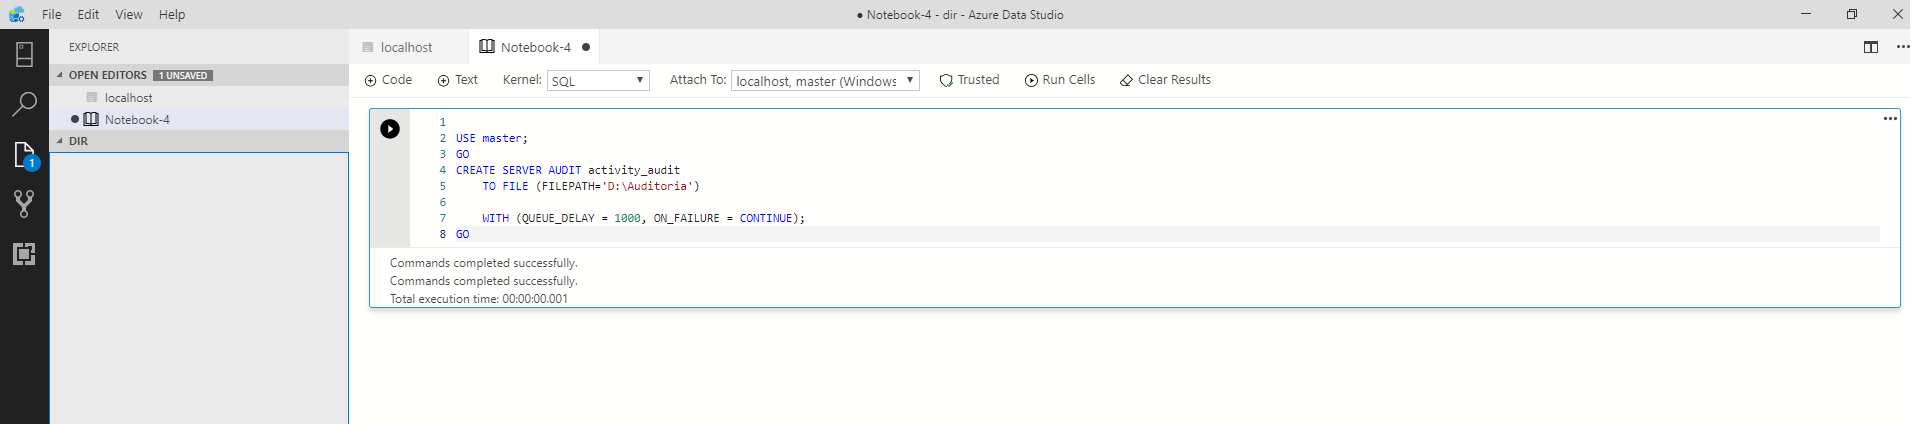
\includegraphics[width=16cm, height=90]{./Imagenes/Imagen1}
   				    \end{center}
   				    
   				    \begin{center}
    				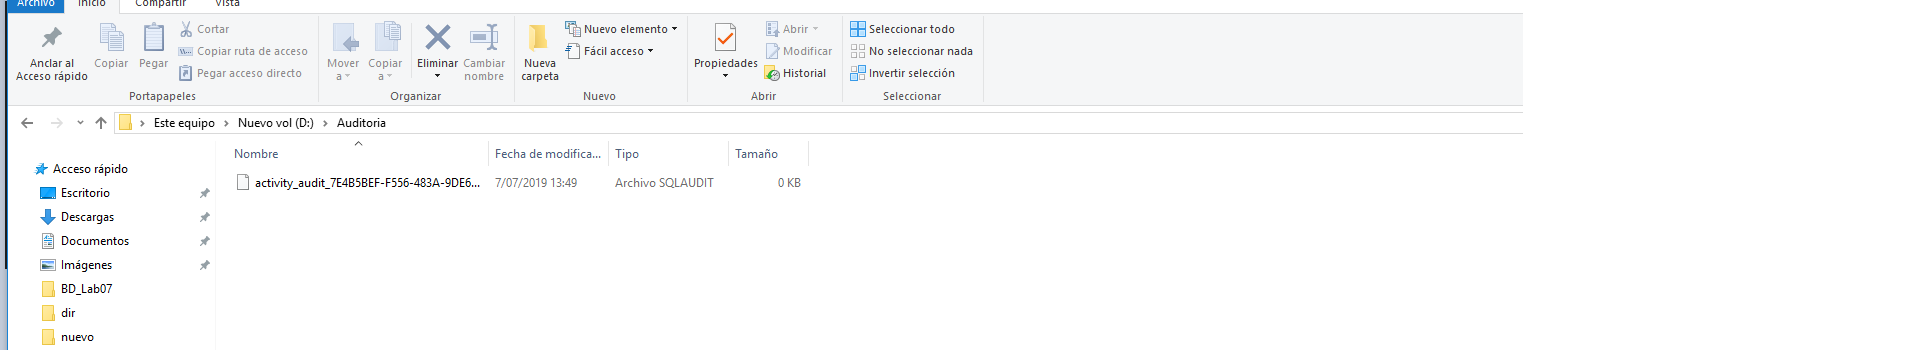
\includegraphics[width=16cm, height=90]{./Imagenes/ImagenAuditoria}
   				    \end{center}
				 

				 \item Paso 2 Activar la auditoria del servidor creada.
				 
				 	\begin{center}
    				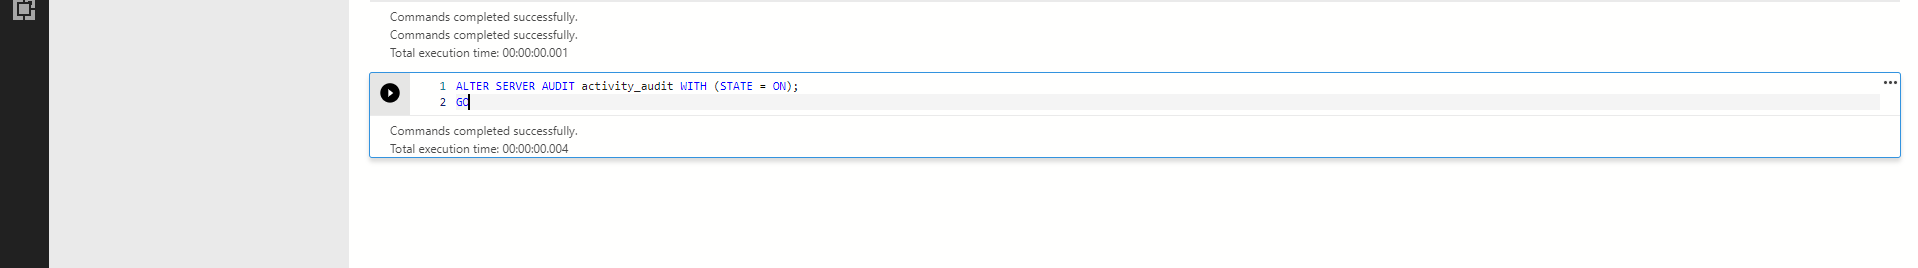
\includegraphics[width=16cm, height=90]{./Imagenes/Imagen2}
   				    \end{center}
				 
				 \item Paso 3 Crear una especificación de auditoría del servidor con las siguientes propiedades.
				 
				 
				 \begin{center}
    				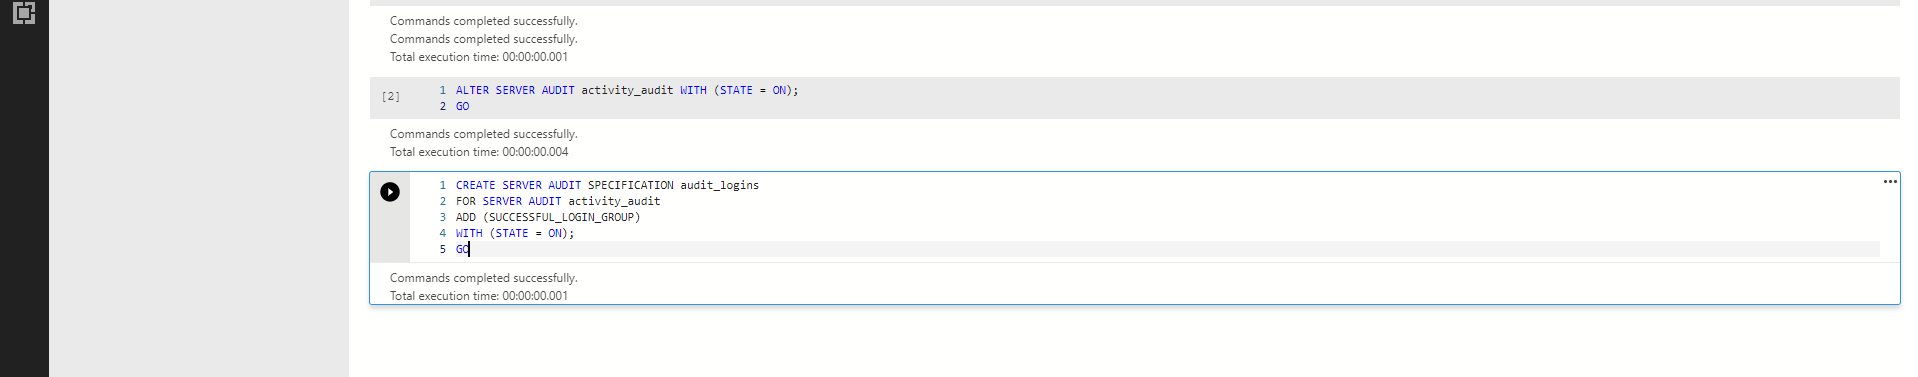
\includegraphics[width=16cm, height=90]{./Imagenes/Imagen3}
   				    \end{center}
				 
				 \item Paso 4 Activar la especificación de auditoria del servidor creada.
				 
				 
				 \begin{center}
    				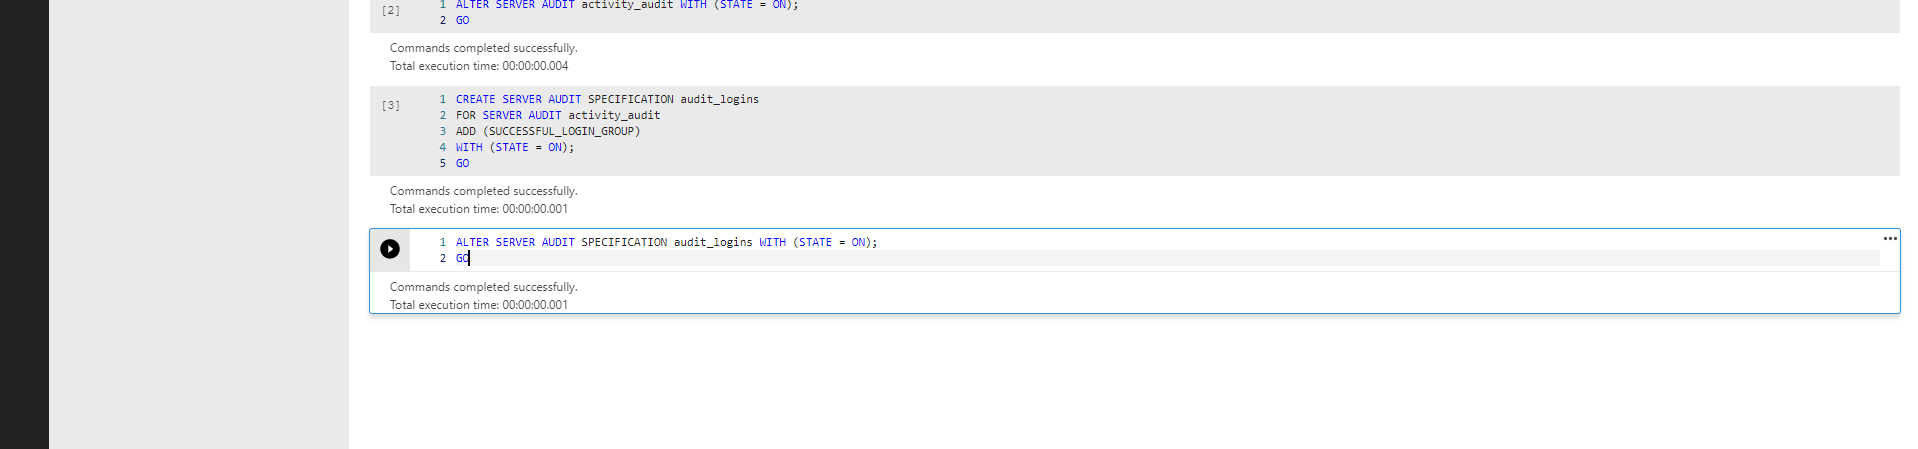
\includegraphics[width=16cm, height=90]{./Imagenes/Imagen4}
   				    \end{center}
   				    	
   				    
   				 \item Paso 5 Crear una especificación de auditoría de base de datos en la base de datos salesapp1 con las siguientes propiedades:
				 
				 
				 \begin{center}
    				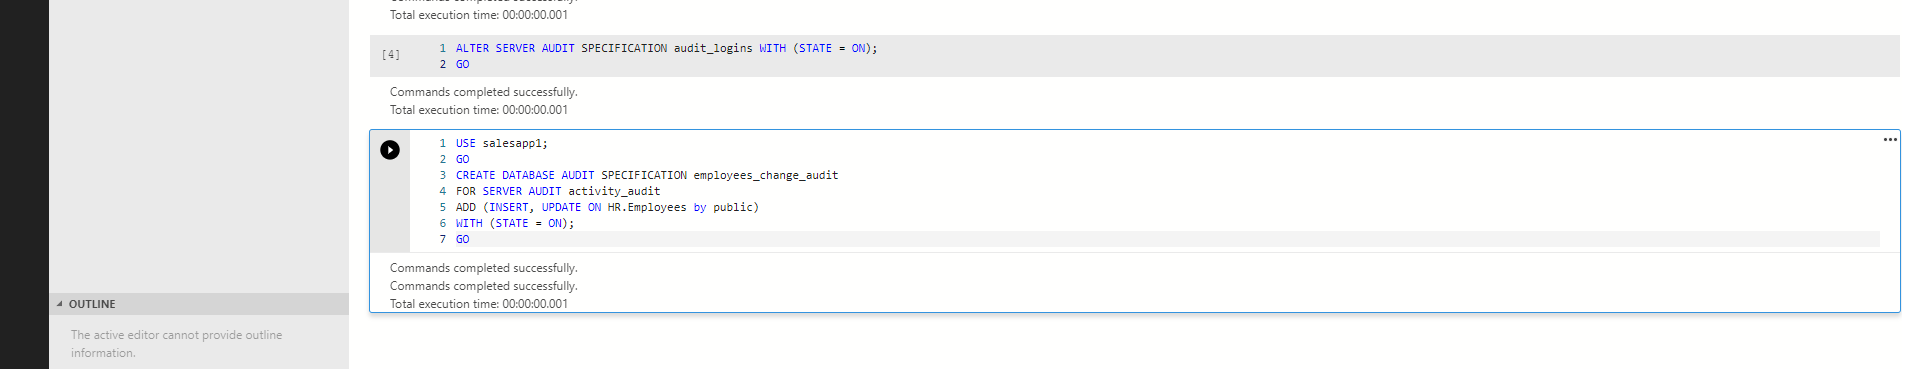
\includegraphics[width=16cm, height=90]{./Imagenes/Imagen5}
   				    \end{center}   		 
				 
				  \item Paso 6 Activar la especificación de auditoría de base de datos creada.
				 
				 \begin{center}
    				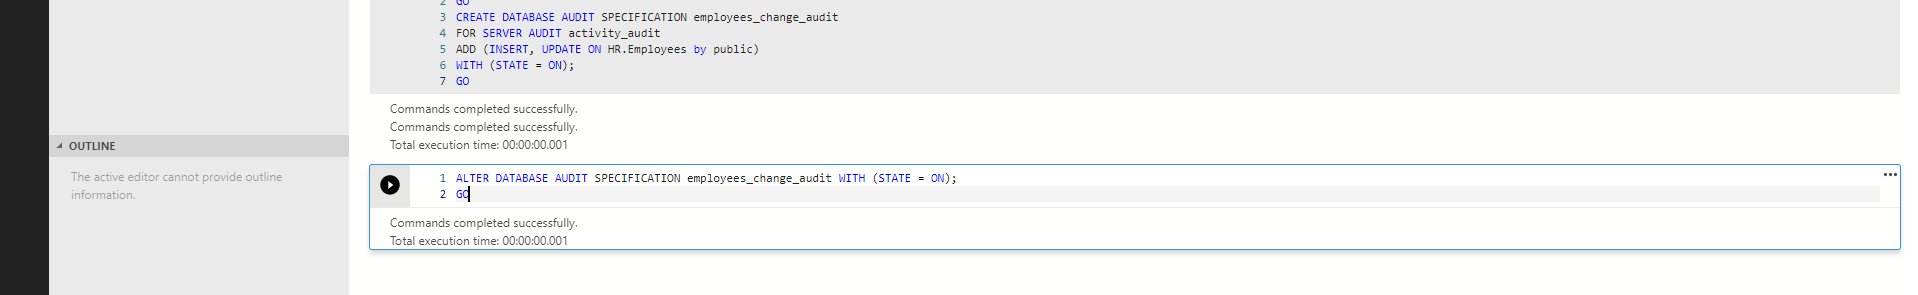
\includegraphics[width=16cm, height=90]{./Imagenes/Imagen6}
   				    \end{center} 
   				    
   				    \item Paso 7 Ejecutar el siguiente código)
				 
				 \begin{center}
    				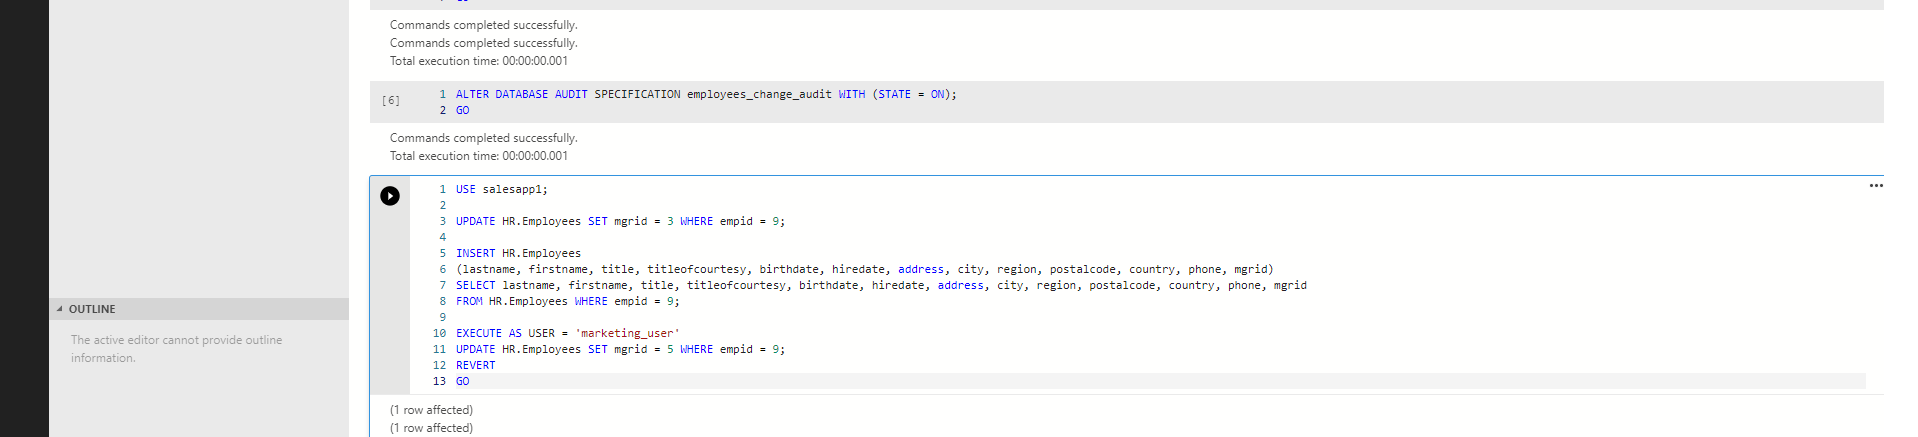
\includegraphics[width=16cm, height=90]{./Imagenes/Imagen7}
   				    \end{center}   
   				    \clearpage
   				    \item Paso 8 Escribir una consulta utilizando la función de sistema sys.fn get audit file para devolver todos los datos de auditoría desde los archivos en D:\Auditoria. Filtrar los datos para que solo la actividad relacionada a la sesión actual sea visualizada.
				 
				 \begin{center}
    				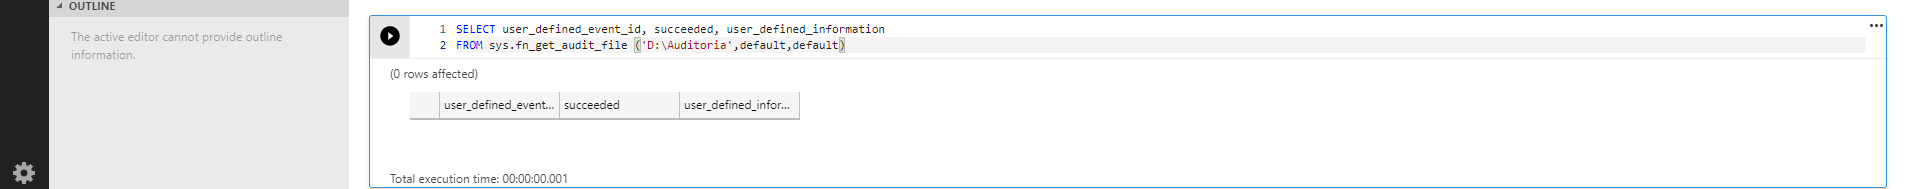
\includegraphics[width=16cm, height=90]{./Imagenes/Imagen8}
   				    \end{center}   
   				    \clearpage	
   				    \item Paso 9 Desahbilitar la auditoría de servidor activity_audit.
				 
				 \begin{center}
    				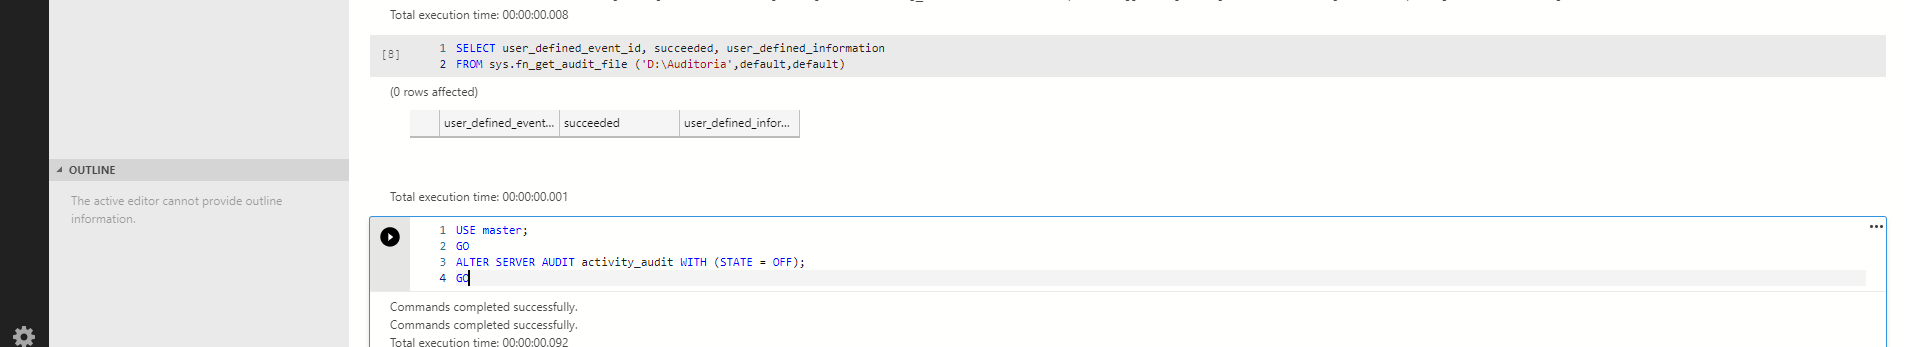
\includegraphics[width=16cm, height=90]{./Imagenes/Imagen9}
   				    \end{center} 	
   				    
   				      
				  
				 				  
				   \end{itemize}
				   \clearpage



\\\\




